\subsection{编写目的}
本文档旨在明确医疗预约管理系统的功能、性能及用户界面需求,确保开发团队与项目管理者对系统需求有统一的理解,并为后续的设计、实施、测试和维护工作提供指导。

\subsection{相关背景}
随着互联网技术的飞速发展,公众对医疗服务的期望不断提升。传统的医疗服务模式已难以满足现代社会对便捷、高效医疗服务的追求。为此,我们提出了医疗预约管理系统项目,旨在通过在线预约、远程问诊、账单管理和用户反馈等功能,提升医疗服务质量和用户体验。

\subsection{项目描述}
\subsubsection{项目提出及意义}
在现代社会的快节奏生活中,公众对医疗服务的需求日益增长。传统的医疗服务方式,例如电话预约和现场排队,已不适应当前的需求。医疗预约管理系统项目利用互联网技术,允许用户随时随地进行医疗服务预约,旨在提高服务效率,减少等待时间,并改善整体用户体验。

\subsubsection{病人功能需求}
本系统致力于为病人提供一个全面、高效的医疗服务体验,通过以下一系列核心功能,确保病人能够轻松管理自己的医疗需求:
\begin{itemize}
	\item 用户注册与登录机制:病人可以通过注册账户并登录系统,以便安全、便捷地使用系统提供的各项服务。
	\item 个人医疗信息管理:用户可以轻松查看、管理和更新自己的个人医疗信息,包括过往病史、药物过敏信息等,以确保信息的准确性和时效性。
	\item 人工智能病情咨询服务:集成AI技术,用户可以咨询自己的病情,并获得初步的医疗建议,为进一步的诊断和治疗提供参考。
	\item 科室与专业领域介绍:系统提供详细的科室信息,包括各科室的专业领域、医生团队介绍等,帮助用户了解并选择合适的科室。
	\item 医生预约时段选择:用户可以查看医生的可选时段,并根据自己的时间安排进行预约,提高就诊的灵活性和便利性。
	\item 医生选择与预约确认:在选定时段后,用户可以根据自己的需求和医生的专业背景选择心仪的医生,并确认预约。
	\item 医疗费用账单管理:用户可以在线提交和查看自己的医疗费用账单,包括详细的费用清单和总计,便于费用的核对和理解。
	\item 缴费与退费流程:系统支持在线缴费和退费功能,简化了费用处理流程,减少了用户在医院的等待时间。
	\item 电子处方查询:用户可以在线查询医生开具的处方信息,包括药物名称、用法用量等,便于用户理解和遵循医嘱。
	\item 电子病历搜索与访问:用户可以搜索并查看自己的电子病历,包括历史就诊记录、检查结果等,便于健康管理和疾病预防。
	\item 预约挂号与问诊服务:用户可以方便地预约挂号,并在预约时间进行在线或线下问诊,确保医疗服务的连续性和及时性。
	\item 时段灵活性与个性化预约:用户可以根据自己的时间安排,选择最佳的就诊时段,系统还会提供个性化的预约建议,以满足不同用户的需求。
	\item 电子问诊单与后续跟进:问诊后,用户可以接收到电子问诊单,便于记录和后续跟进,确保医疗服务的完整性。
	\item 医疗服务评价体系参与:用户可以参与对医生和医院服务的评价,为其他患者提供参考,同时也帮助医疗机构改进服务质量。
	\item 处方与病历的综合查询:用户可以查询医生开具的处方,并访问自己的电子病历,便于对健康状况进行全面管理。
\end{itemize}

通过这些功能,系统旨在为病人提供一个无缝、高效的医疗服务体验,从而提高医疗服务的可及性和效率,确保用户能够享受到高质量的医疗服务。这不仅能够提升病人的满意度,还能够促进医疗服务的整体改进和发展。

\subsubsection{项目研究现状}
随着数字化和网络化技术的不断进步,中国的医疗行业正在经历一场深刻的转型。虽然一些大型医疗机构已经开始引入在线预约系统,但这些系统大多数仅服务于单一机构,未能实现全面的互联互通。与此同时,中小型医疗机构由于技术和资金的限制,尚未能广泛开展在线服务。因此,开发一个全面、一体化的医疗预约管理系统对于提高医疗服务效率、实现资源共享具有重大意义。

在国内外,已有多个在线预约诊疗服务平台开始运营,如\href{http://www.zjol.com.cn}{浙江在线预约诊疗服务平台}和\href{http://www.wedoctor.com}{微医-互联网医院在线诊疗平台}。这些平台为病人提供了一站式的医疗服务,包括注册、登录、查看个人信息、AI病情咨询、科室浏览、医生预约、账单提交与缴费等。此外,病人还可以参与到问诊评价体系中,为医疗服务提供反馈。

\begin{figure}[htbp]
	\centering
	\begin{minipage}[b]{0.5\textwidth}
		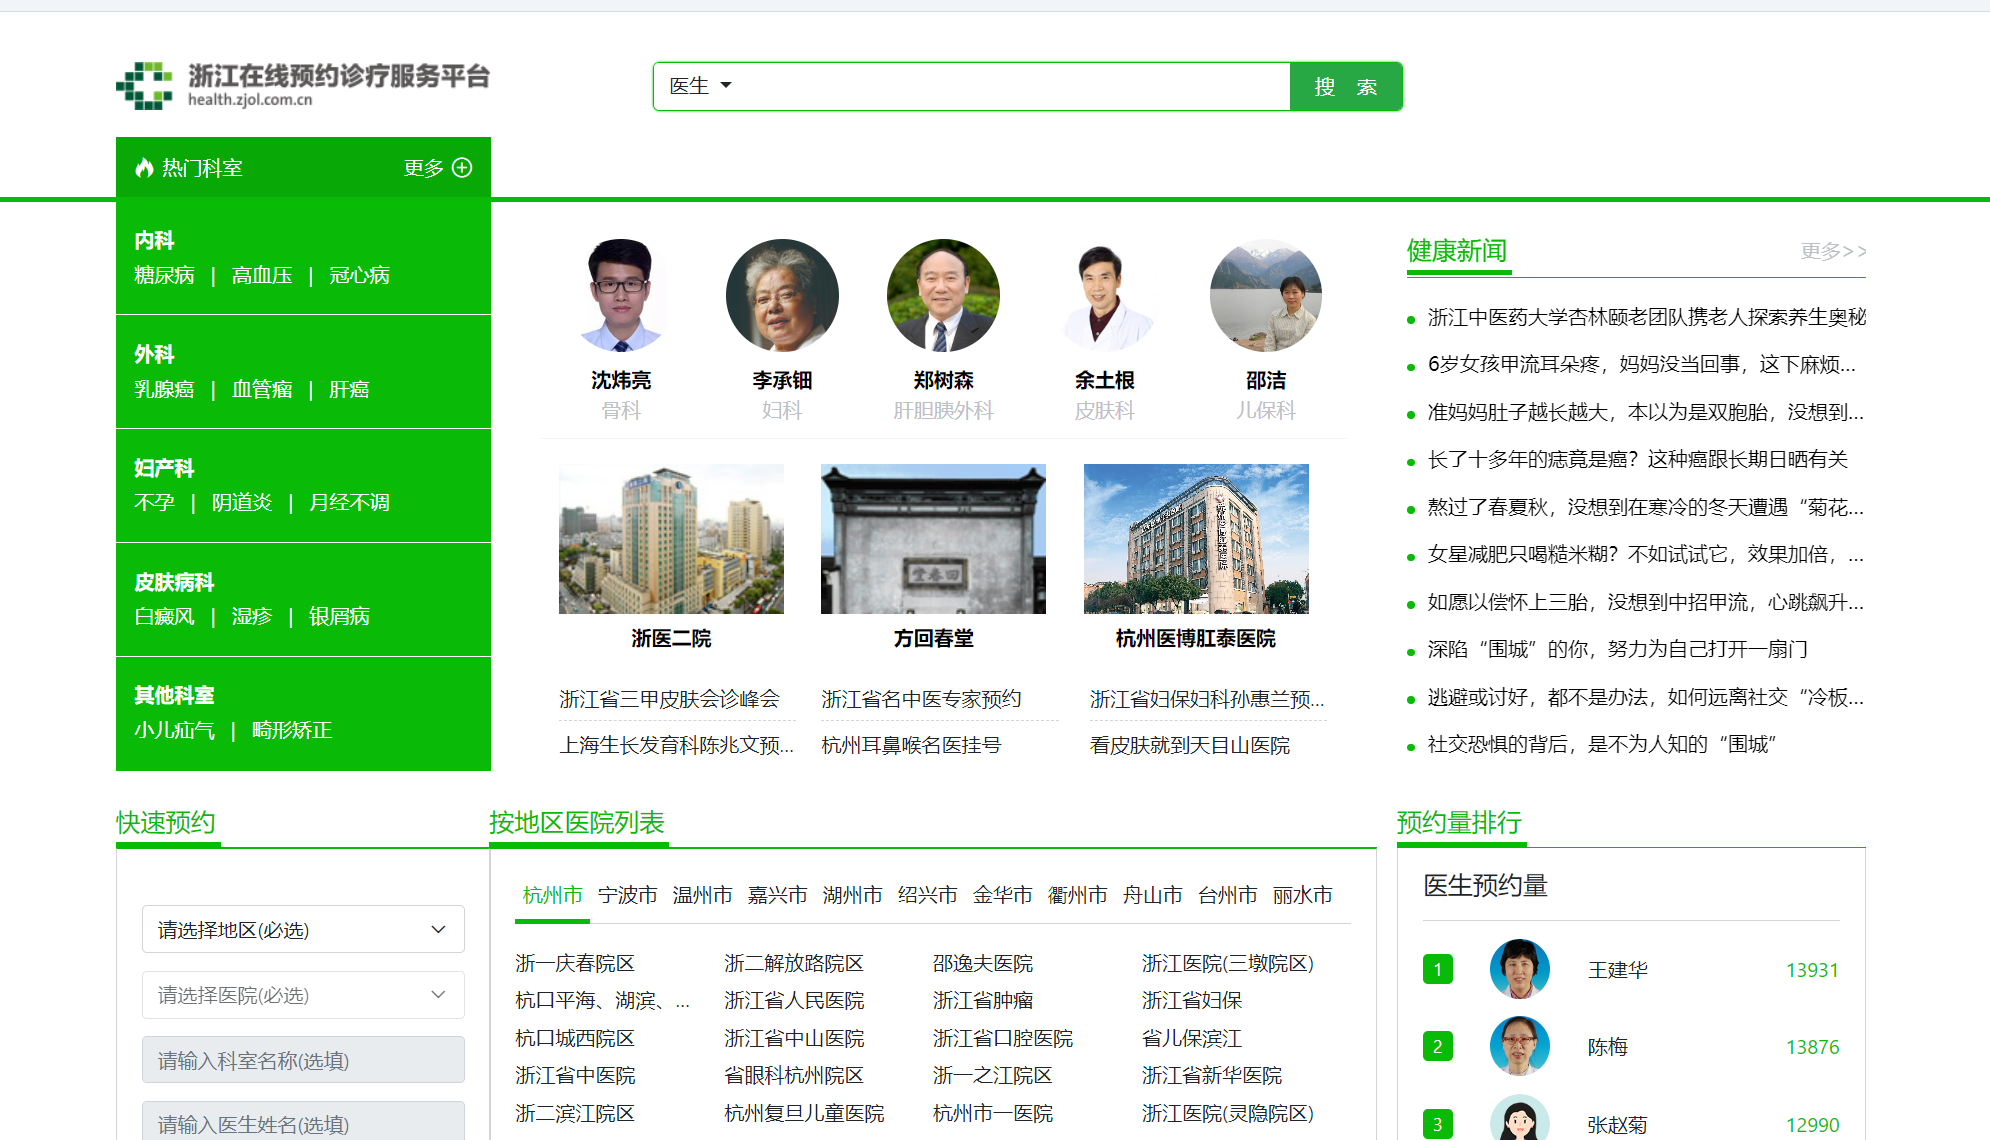
\includegraphics[width=\textwidth]{figures/01.png} % 假设图片文件名为01.png
		\caption{浙江在线预约诊疗服务平台}
	\end{minipage}%
	\begin{minipage}[b]{0.5\textwidth}
		
\includegraphics[width=\textwidth]{figures/02.png} % 假设图片文件名为02.png
		\caption{微医-互联网医院在线诊疗平台}
	\end{minipage}
	% 两个minipage并排放置
\end{figure}

对于病人而言,一个高效、易用的\textbf{医疗预约管理系统}应当具备以下功能:预约挂号、退号、费用查询、缴费退费、查询处方和搜索相关病历等。这些功能的实现将极大地提升病人的医疗服务体验,使得病人能够更加便捷地获取医疗服务。

\subsubsection{国外研究现状}
放眼全球,许多国家的医疗机构已经成功实施了在线预约和服务模式,例如美国的Zocdoc和英国的NHS App。这些平台通过互联网技术显著提升了医疗服务的便捷性和效率。然而,这些系统多为英文界面,对于非英语使用者可能存在一定的使用障碍。因此,针对国内语言和文化特色开发医疗预约管理系统,以更好地满足国内患者的实际需求,显得尤为迫切和重要。

综上所述,一个综合性的医疗预约管理系统不仅能够提高医疗服务的可及性和效率,还能够为病人带来更加人性化的服务体验。通过实现预约挂号、问诊、基本信息查询等功能,系统将极大地简化病人的医疗服务流程,提升整体医疗服务质量。